\section{Short introduction}



\section{Main simulation panel}
This panel is the main part of the simulator user interface.
You can see status of internal registers, scratchpad ram, input and output ports, stack, program counter, elapsed time and cycles, actual clock and internal flags: CARRY and ZERO. All those features can be edited during processor simulation.

   \begin{figure}[h!]
        \centering
        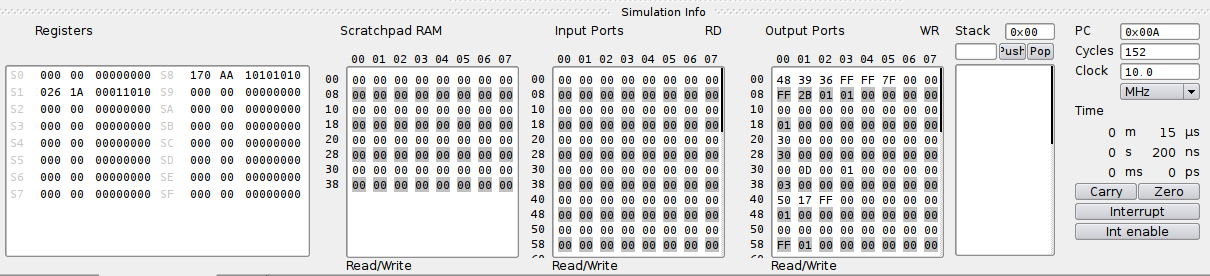
\includegraphics[width=\textwidth]{img/bottom_panel.png}
        \caption{Main simulator panel}
    \end{figure}

   \begin{figure}[h!]
        \centering
        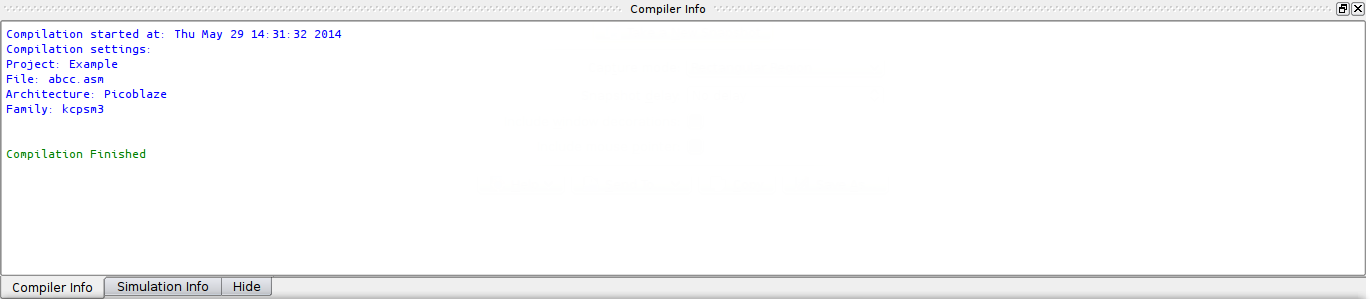
\includegraphics[width=\textwidth]{img/compiler_panel.png}
        \caption{Compiler info panel}
    \end{figure}

\section{List of macros and symbols}
% warningy dodelat
    \begin{table}[h!]
        \begin{tabular}{cc}
            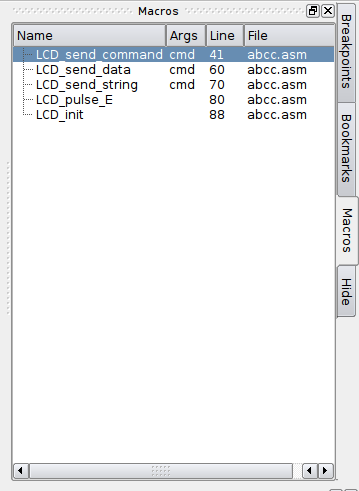
\includegraphics[width=.33\textwidth]{img/macro_panel.png}
                &
            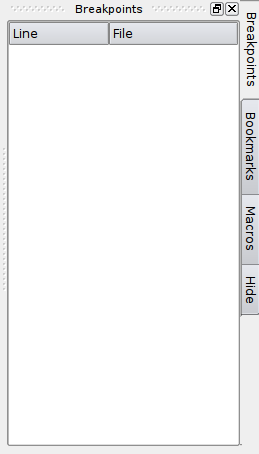
\includegraphics[width=.33\textwidth]{img/right_panel.png}
                \\
            Macros & Breakpoints
        \end{tabular}
    \end{table}

    
\section{Modes of simulation}
    There are 4 modes of simulation:

    \begin{figure}[h!]
        \centering{}
        
\includegraphics[width=.4\textwidth]{img/simulation_panel.png}
        \caption{Simulator toolbar.}
    \end{figure}
    
    \begin{itemize}
        \item STEP: Execute exactly one intruction, no matter how many machine cycles it will take. This does not apply for macro-instruction, in that case each instruction of the macro is executed separately.
        \item ANIMATE: Do the same as step, but in a loop, one after another until stopped by a waring condition or user request.
        \item RUN: This is generally the same as animate, but much faster, because GUI is not updated so often as in the animate mode.
        \item RESET: Resets everything to the initial state of program.
        \item UNHIGHLIGHT: Cleans up all highlighted text.
    \end{itemize}
